\documentclass[12pt]{article}
\usepackage{graphicx}
\usepackage{amsmath}
\usepackage{mathtools}
\usepackage{gensymb}

\newcommand{\mydet}[1]{\ensuremath{\begin{vmatrix}#1\end{vmatrix}}}
\providecommand{\brak}[1]{\ensuremath{\left(#1\right)}}
\providecommand{\norm}[1]{\left\lVert#1\right\rVert}
\newcommand{\solution}{\noindent \textbf{Solution: }}
\newcommand{\myvec}[1]{\ensuremath{\begin{pmatrix}#1\end{pmatrix}}}
\let\vec\mathbf

\begin{document}
\begin{center}
\textbf\large{CHAPTER-7 \\ COORDINATE GEOMETRY}

\end{center}
\section*{Excercise 7.1}

Q6. Name the type of quadilateral formed,if any, by the following points, and give reasons for your answer:
\begin{enumerate}
	\item $\brak{-1,-2}, \brak{1,0}, \brak{-1,2}, \brak{-3,0}$ 
	\item $\brak{-3,5}, \brak{3,1}, \brak{0,3}, \brak{-1,-4}$
	\item $\brak{4,5}, \brak{7,6}, \brak{4,3}, \brak{1,2}$
\end{enumerate}
\solution
\begin{enumerate}
\item The coordinates are given as
	\begin{align}
	\vec{A} = \myvec{
		-1\\
		-2\\
		},
	\vec{B} = \myvec{
		1\\
		0\\
		},
	\vec{C} = \myvec{
		-1\\
		2\\
		} \text{ and }
	\vec{D} = \myvec{
		-3\\
		0\\
		}
	\end{align}
	\begin{align}
		AB &= \vec{B} - \vec{A} = \myvec{1\\0} - \myvec{-1\\-2} = \myvec{2\\2}\\
		BC &= \vec{C} - \vec{B} = \myvec{-1\\2} - \myvec{1\\0} = \myvec{-2\\2}\\
		DC &= \vec{C} - \vec{D} = \myvec{-1\\2} - \myvec{-3\\0} = \myvec{2\\2}\\
		AD &= \vec{D} - \vec{A} = \myvec{-3\\0} - \myvec{-1\\-2} = \myvec{-2\\2}\\
		AC &= \vec{C} - \vec{A} = \myvec{-1\\2} - \myvec{-1\\-2} = \myvec{0\\4}\\
		BD &= \vec{D} - \vec{B} = \myvec{-3\\0} - \myvec{1\\0} = \myvec{-4\\0}
	\end{align}
	If rank of $\myvec{AB & DC} < 2$ then AB is parallel to DC else it is not.\\
	$\text{Rank of } \myvec{AB & DC} = \text{Rank of }\myvec{2&2\\2&2}$\\
	$\text{Rank } = 1$\\
	Hence, AB is parallel to DC\\
	Similarly,If rank of $\myvec{BC & AD} < 2$ then BC is parallel to AD else it is not.\\
	$\text{Rank of } \myvec{BC & AD} = \text{Rank of }\myvec{-2&-2\\2&2}$\\
	$\text{Rank } = 1$\\
	Hence, BC is parallel to AD\\
	From here we can conclude that ABCD is parallelogram.\\
	Now checking if the adjacent sides are orthogonal to each other
	\begin{align}
		(AB)^\top (BC) = \myvec{2&2} \myvec{-2\\2} = -4+4 = 0
	\end{align}
	Now if the diagonals are also orthogonal then it is a square else a rectangle
	\begin{align}
		(AC)^\top (BD) = \myvec{0&4} \myvec{-4\\0} = 0
	\end{align}
	Hence the diagonals are orthogonal to each other.
	So, we can conclude that ABCD is a square as shown in Figure \ref{fig:Fig1}
 
\begin{figure}[!h]
	\begin{center} 
	    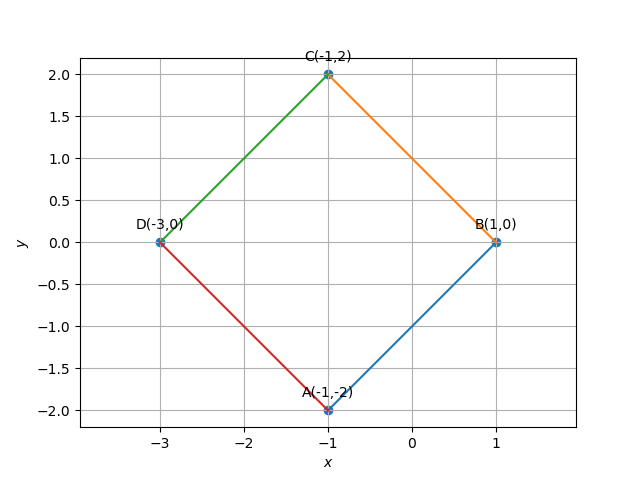
\includegraphics[width=\columnwidth]{./quad1.png}
	\end{center}
\caption{}
\label{fig:Fig1}
\end{figure}

\item The coordinates are given as
	\begin{align}
	\vec{A} = \myvec{
		-3\\
		5\\
		},
	\vec{B} = \myvec{
		3\\
		1\\
		},
	\vec{C} = \myvec{
		0\\
		3\\
		} \text{ and }
	\vec{D} = \myvec{
		-1\\
		-4\\
		}
	\end{align}
	\begin{align}
		AB &= \vec{B} - \vec{A} = \myvec{3\\1} - \myvec{-3\\5} = \myvec{6\\-4}\\
		BC &= \vec{C} - \vec{B} = \myvec{0\\3} - \myvec{3\\1} = \myvec{-3\\2}\\
		DC &= \vec{C} - \vec{D} = \myvec{0\\3} - \myvec{-1\\-4} = \myvec{1\\7}\\
		AD &= \vec{D} - \vec{A} = \myvec{-1\\-4} - \myvec{-3\\5} = \myvec{2\\-9}\\
		AC &= \vec{C} - \vec{A} = \myvec{0\\3} - \myvec{-3\\5} = \myvec{3\\-2}\\
		BD &= \vec{D} - \vec{B} = \myvec{-1\\-4} - \myvec{3\\1} = \myvec{-4\\-5}
	\end{align}
	If rank of $\myvec{AB & DC} < 2$ then AB is parallel to DC else it is not.\\
	$\text{Rank of } \myvec{AB & DC} = \text{Rank of }\myvec{6&-1\\-4&7}$\\
	$\text{Rank } = 2$\\
	Hence, AB is not parallel to DC\\
	Similarly,If rank of $\myvec{BC & AD} < 2$ then BC is parallel to AD else it is not.\\
	$\text{Rank of } \myvec{BC & AD} = \text{Rank of }\myvec{-3&2\\2&-9}$\\
	$\text{Rank } = 2$\\
	Hence, BC is not parallel to AD\\
	Now to check if any three points are co-linear\\
	if rank of $\myvec{AB & BC} < 2$ then points are co-linear\\
	$\text{Rank of }\myvec{AB & BC} = \text{Rank of }\myvec{6&-3\\-4&2}$\\
	$\text{Rank } = 1$\\
	Since none of the opposite sides are parallel to each other and three points are co-linear so these does not form a quadilateral as shown in Figure \ref{fig:Fig2}\\
	
\begin{figure}[!h]
	\begin{center} 
	    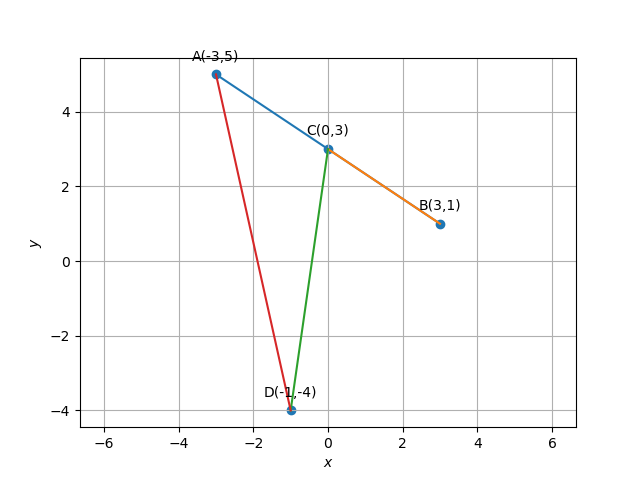
\includegraphics[width=\columnwidth]{./quad2.png}
	\end{center}
\caption{}
\label{fig:Fig2}
\end{figure}
	
\item The coordinates are given as
	\begin{align}
	\vec{A} = \myvec{
		4\\
		5\\
		},
	\vec{B} = \myvec{
		7\\
		6\\
		},
	\vec{C} = \myvec{
		4\\
		3\\
		} \text{ and }
	\vec{D} = \myvec{
		1\\
		2\\
		}
	\end{align}
	\begin{align}
		AB &= \vec{B} - \vec{A} = \myvec{7\\6} - \myvec{4\\5} = \myvec{3\\1}\\
		BC &= \vec{C} - \vec{B} = \myvec{4\\3} - \myvec{7\\6} = \myvec{-3\\-3}\\
		DC &= \vec{C} - \vec{D} = \myvec{4\\3} - \myvec{1\\2} = \myvec{3\\1}\\
		AD &= \vec{D} - \vec{A} = \myvec{1\\2} - \myvec{4\\5} = \myvec{-3\\-3}\\
		AC &= \vec{C} - \vec{A} = \myvec{4\\3} - \myvec{4\\5} = \myvec{0\\-2}\\
		BD &= \vec{D} - \vec{B} = \myvec{1\\2} - \myvec{7\\6} = \myvec{-6\\-4}
	\end{align}
	If rank of $\myvec{AB & DC} < 2$ then AB is parallel to DC else it is not.\\
	$\text{Rank of } \myvec{AB & DC} = \text{Rank of }\myvec{3&3\\1&1}$\\
	$\text{Rank } = 1$\\
	Hence, AB is parallel to DC\\
	Similarly,If rank of $\myvec{BC & AD} < 2$ then BC is parallel to AD else it is not.\\
	$\text{Rank of } \myvec{BC & AD} = \text{Rank of }\myvec{-3&-3\\-3&-3}$\\
	$\text{Rank } = 1$\\
	Hence, BC is parallel to AD\\
	From here we can conclude that ABCD is parallelogram.\\
	Now checking if the adjacent sides are orthogonal to each other
	\begin{align}
		(AB)^\top (BC) = \myvec{3&1} \myvec{-3\\-3} = -9-3 = -12
	\end{align}
	Since inner product is not zero so AB and BC are not orthogonal.\\
	Hence, we can say that ABCD is neither a rectangle nor a square.\\
	Now if the diagonals are also orthogonal then it is a Rhombus
	\begin{align}
		(AC)^\top (BD) = \myvec{0&-2} \myvec{-6\\-4} = 0+8 = 8
	\end{align}
	Hence the diagonals are also not orthogonal so we conclude that ABCD is a parallelogram as shown in Figure \ref{fig:Fig3}

\begin{figure}[!h]
	\begin{center} 
	    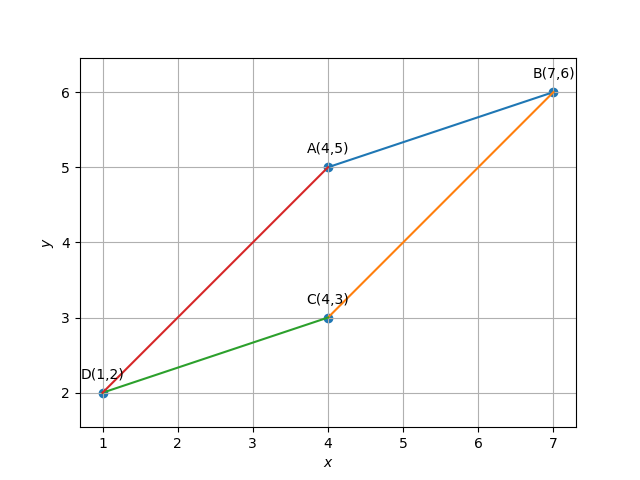
\includegraphics[width=\columnwidth]{./quad3.png}
	\end{center}
\caption{}
\label{fig:Fig3}
\end{figure}
\end{enumerate}














\end{document}

